\begin{savequote}[75mm]
Figure out who you are and do it on purpose.
\qauthor{Dolly Parton}
\end{savequote}

\chapter{Machine Learning}

Machine Learning (ML) encompasses a variety of statistical techniques and models that allow algorithms to learn patterns and behaviors without being explicitly programmed. The study and development of these techniques has been on-going since the 1960s, however the subset of ML called Deep Learning (DL) which allowed effective training of very large, complex algorithms over high-dimensionality data-sets only emerged in 2012 \cite{nips_2012}. Today, DL, and more broadly ML, is used to solve complex computing problems in a variety of fields including image processing (\cite{medical_img} \cite{img_cap}), language processing (\cite{nlp1} \cite{nlp2}), resource distribution \cite{resource_dist}, security \cite{security1}, and content personalization \cite{personalization}.\\

In many ways, ML and physics share similar goals: building mathematical models to fit a set of observations and making predictions in related environments using those models. Given these shared goals and the complex and intensive computing needs of LHC experiments (Chapter 3), it is no surprise that ML for HEP has evolved into its own field of research. This chapter describes the current status of these efforts: important ML concepts are defined in Section \ref{sec:concepts} commonly used algorithms are introduced in Section \ref{sec:algs} and novel applications in HEP are presented in Section \ref{sec:apps}.\\

%% SEC: ALGORITHMS
\section{Central Concepts}\label{sec:concepts}
ML tasks can be separated into two classes. Supervised learning methods are used to map input data to a discrete set of labels or some continuous output distribution; they are developed using data-sets where the ground truth (i.e. the correct classification of a data point) is known. Unsupervised learning methods aim to infer natural structure within the input data and are developed without any ground truth information. Much of the current research on ML for HEP utilizes supervised learning and so the remainder of this chapter will focus only on supervised algorithms.\\

Supervised learning tasks typically take the form of a search for a function $f: \textbf{X}\rightarrow \textbf{Y}$ which maps the input data \textbf{X} (also called training data) to a lower-dimensional space of target labels \textbf{Y} with a primary goal of minimizing the loss function $L(\mathbf{y},f(\mathbf{x}))$. The specific form of the loss function depends on the individual task, the selected algorithm, and the training procedure. Common, appropriate loss functions are included in the algorithm descriptions in the following sections.\\  

In an ideal case, the ML algorithm would find the function $f$ that minimizes $L$ over all possible values of $(\mathbf{x},\mathbf{y})$. In practice, however, this is impossible with current computing architectures due to the high dimensionality of typical training data-sets and the enormous allowed function space. Thus, the algorithm training procedure seeks to minimize $L$ over the training data-set values within a reduced function space $f_{\phi}$ defined by algorithm-specific parameters $\phi$.\\

The performance of a trained ML algorithm can be evaluated using a range of criteria and selecting a task appropriate evaluation metric is a critical part of ML design. One of the most common evaluation methods for classification algorithms is the Confusion Matrix \cite{confusion_matrix}, an $\text{N}\times\text{N}$ matrix where N is the number of class labels. The matrix values $(n,m)$ represent the number of data points whose ground truth is $n$ and predicted label is $m$. This leads to several easily commutable evaluation metrics like accuracy (percentage of correct predictions), class precision (the percentage of a predicted class whose ground truth is the same label), and class sensitivity (the percentage of a ground truth class whose predicted labels are correct). In binary classification tasks, the Confusion Matrix can be used to construct the Receiver Operating Characteristic curve (ROC curve) which plots the positive class sensitivity vs 1-negative class sensitivity. The area under the ROC curve (AUC-ROC) serves as an additional evaluation metric; the closer the AUC-ROC is to one, the better the performance.\\

The ultimate goal of a trained (supervised) ML algorithm is to perform well on new data not encountered during the training process; this is referred to as generalization and a failure to do this is called over-training to indicate that the algorithm has learned non-generalizable information present only in the training data. Over-training is often only identified by running the trained algorithm over a portion of the input data that was not used for training (called a test set); thus, test set validation is a critical component of ML model design. Test set validation can be incorporated directly into training through the method of cross-validation \cite{cross-val}, where the algorithm is trained multiple times with a different randomized subset of training data (validation set) omitted each time; the validation set is used to quantify the error for that particular trained model and the final algorithm is an average of the various models.\\ 

Additionally, a variety of techniques can be used to reduce the risk of over-training, collectively referred to as regularization methods \cite{regularization}. These are generally incorporated into the loss function formulation and penalize the algorithm for having large function parameters. They can also take the form of drop-out methods that randomly set some function parameters to zero. Increasing the size of the training data-set is another way to reduce the risk of over-training, but this increases the required computing time to train the algorithm.\\ 

Algorithm optimization often involves tuning specific meta-variables called hyperparameters. These include the learning rate (what amount the function parameters are adjusted in each training iteration (epoch)), drop-out rate, regularization weight (how important the regularization goal is compared to other components of the loss function), initialization of the function parameters, and other task specific parameters. The most common method for tuning hyperparameters is a grid search where the model is trained multiple times where the hyperparameters are selected from an N$\times$M matrix that gives $n$ possible values for each of $m$ hyperparameters.

\section{Algorithms}\label{sec:algs}
HEP utilizations of ML generally implement one of two algorithm types: Boosted Decisions Trees (BDTs) and Artificial Neural Networks (NNs). The basics construction and training procedures for each are outlined in the following sections. For all algorithms, the variables represented in the training data-set are referred to as features.

%subsec: BDTS
\subsection{Boosted Decision Trees}
The fundamental component of a BDT is a decision tree as shown in Figure \ref{fig:dt_diag}. Decision trees can be constructed algorithmically for class labeling tasks according to the following steps:
\begin{enumerate}
    \item All data (containing examples of all classes) is equally weighted and input at the root node.
    \item At each branching, all possible linear cuts on all features are considered and the cut that best separates one class from the rest of the data is selected.
    \item Step 2 is continued until a stopping criteria is reached (typically when a node has fewer than x data points or the tree reaches some specified depth).
    \item For each final node, the label of the the class with the most (ground truth labeled) data points in that node is assigned to all data points in that node.
\end{enumerate}
\noindent Although simple to understand, an individual decision tree does not typically achieve high levels of accuracy.\\

\begin{figure}[htb!]
    \centering
    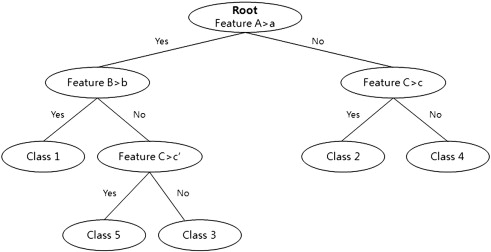
\includegraphics[width=4in]{figures/chapter4/dt_diag.jpg}
    \caption{Depiction of an algorithmically constructed decision tree.}
    \label{fig:dt_diag}
\end{figure}

In ML, an ensemble method is an algorithm that iteratively combines weak learners to form a single strong learner. A BDT is then an ensemble method that applies `boosting' to a `forest' of decision trees . This method was first developed in 1995 in an effort to conceptualize decision trees as an ML optimization problem with a loss function, generally the mean squared error $L=\frac{1}{n}\sum_i(y_{i}-
\hat{y}_{i})$ for a data-set of size $n$ with $i$ truth labels $y_{i}$ and learned labels $\hat{y}_i$ \cite{bdt_paper}. Boosting describes the training procedure of not retraining the individual tree but instead creating a new tree where the previously mis-classified data-points are given a higher weight in the root node. All the trees are then combined to create the final model and the loss function is evaluated over this ensemble; this process is demonstrated in Figure \ref{fig:bdt_diag}. There are a variety of different boosting methods, but gradient boosting, as described in \cite{gradient_boosting}, is the most common.\\

\begin{figure}[htb!]
    \centering
    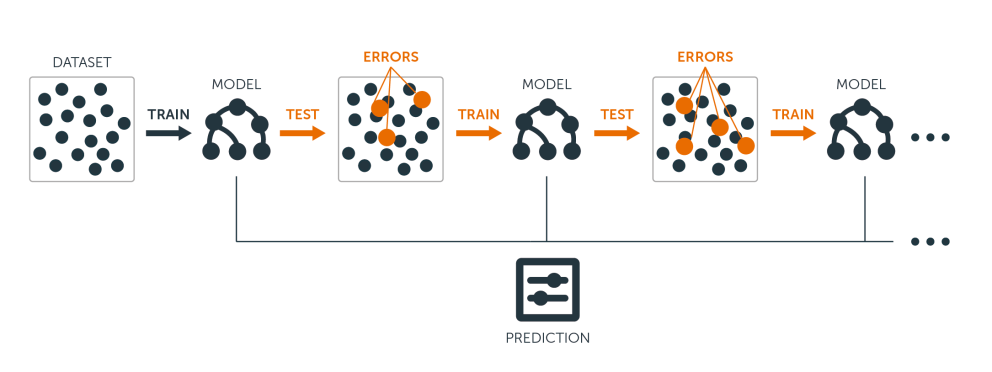
\includegraphics[width=5in]{figures/chapter4/bdt_diag.png}
    \caption{Schematic diagram of a boosted forest of decision trees \cite{bdt_figure}.}
    \label{fig:bdt_diag}
\end{figure}

BDTs are preferred in some HEP ML tasks because they are relatively easy to construct, tend to perform well with little optimization, and are faster to train than most other algorithms. Additionally, the classification decisions are easy to understand, and least for each individual tree. On the other hand, BDTs are highly prone to over-training, particularly if the training data is high dimensional. Consequently, developing BDTs for HEP tasks often necessitates intensive feature-engineering where physicists construct training variables to preserve maximal information with limited dimensionality. Additionally, there are several regularization methods which are applicable to BDTs including shrinkage (where the up-weighting of mis-classified data points is reduced as the number of trees grows). 

%subsec: NNs
\subsection{Neural Networks}
NNs are ML algorithms whose data processing methods were inspired by the brain's biological neural network. NNs consist of `artificial neurons' called nodes arranged in a layered structure. Information is transmitted between layers through series of weighted connections (based on neural synapses). These connections can be represented as a matrix whose values are the connection weights. Learning appropriate weights to model the input data is the primary goal of NN training. A simple fully-connected NN architecture is shown in Figure \ref{fig:nn_diag}; the first layer is composed of input nodes with one for each feature of the training data, the middle layers are called hidden layers, and the final layer is composed of output nodes which give the final results (e.g. predicted label in classification tasks) \cite{nn_paper}.\\

\begin{figure}[htb!]
    \centering
    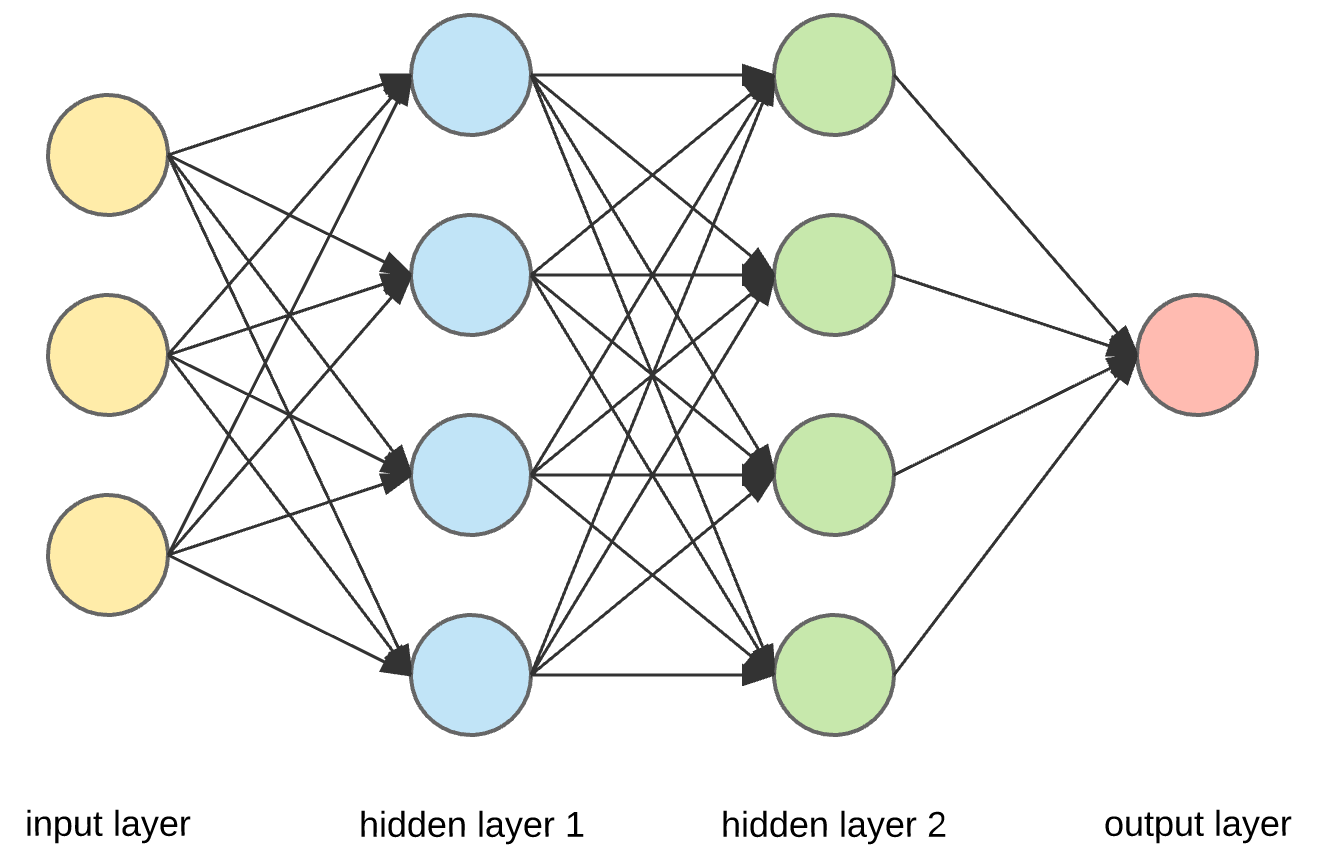
\includegraphics[width=4in]{figures/chapter4/nn_diag.png}
    \caption{Schematic diagram of a simple fully-connected neural network.}
    \label{fig:nn_diag}
\end{figure}

In contrast to BDTs, NNs create a non-linear transformation of the input data because each node has an activation function. Like neural synapses, these activation functions allow information to be transmitted between nodes only if a certain threshold is reached. Mathematically the transformations between layers ($\mathbf{h}$) is formulated as
$$
\mathbf{h}_{i+1}=g_i(W_i\mathbf{h}_i+\mathbf{b})
$$
\noindent where $g_i$ is the activation function for that layer, $W_i$ is the matrix of connection weights, and $\mathbf{b}_i$ is an optional vector of biases which would also be learned during training. Common activation functions include step functions, sigmoids, tanh, and Rectified Linear Units (ReLu) of the form $R(x)=\text{max}(0,x)$.\\

Common loss functions for NNs include Mean Squared Error, Mean Squared Logarithmic Error, Mean Absolute Error, Cross-Entropy 
($L=\frac{1}{n}\sum_i^{i=n}[y_{i}\text{log}(\hat{y}_i+(1-y_i)\text{log}(1-\hat{y}_i]$), and Negative Logarithmic Likelihood ($L=-\frac{1}{n}\sum_i^(i=n)\text{log}(\hat{y}_i)$). The choice of loss function ultimately depends on the training task and the chosen activation function.\\

NNs are trained using a method called backpropagation \cite{backprop}:
\begin{enumerate}
    \item The NN weights are randomly initialized.
    \item The training data is processed through the initial NN.
    \item The predicted output values are compared to the ground truth values and the resulting error is calculated according to the the loss function.
    \item The NN weights are adjusted to reduce the value of $L$.
    \item Steps 1-4 are repeated until some stopping criteria is reached (typically number of epochs or minimal variation in $L$ over several epochs).
\end{enumerate}
\noindent The weight updates in the backpropagation training process is typically done using stochastic gradient descent:
$$
w_{ij}(e+1)=w_{ij}(e)-r\frac{\partial L}{\partial w_{ij}}-\zeta(e)
$$
\noindent where $e$ indicates the epoch, $r$ is the learning rate and $\zeta$ is a stochastic term. This requires that the loss function is differentiable.\\

In practice, deep NNs (containing many hidden layers) often encounter the so-called `vanishing gradient problem' \cite{vanishing_gradient}: as the error is backpropagated through the layers, the gradient rapidly approaches zero making it difficult to improve model performance. In recent years several computing innovations have been developed that allow for accurate training of very deep NNs. These include additional computing power from GPUs, dropout, and pre-training to initialize the network weights with e.g. autoencoders \cite{autoencoders}.\\

In addition to the basic structure outlined above, deep NNs can contain other modular differentiable components. The most common such components are convolutional filters and recurrent units, both of which are described below.

\subsubsection{Convolutional NNs}
The development of convolutional NNs (CNNs) was transformative for ML based image processing \cite{cnn_paper}. Training images are represented as 2D matrices of pixel values. The primary component of a CNN is a convolutional layer that applies a set of learnable filters as convolutions to the training data. Each filter is applied to a small portion of the input and then passed as a sliding window over the width and height (and depth in the case of 3D convolutions) of the input. This tiling allows the filter to learn information about the image regardless of rotations or distortions. An example of an individual convolutional filter is shown in Figure \ref{fig:conv}.\\

\begin{figure}[htb!]
    \centering
    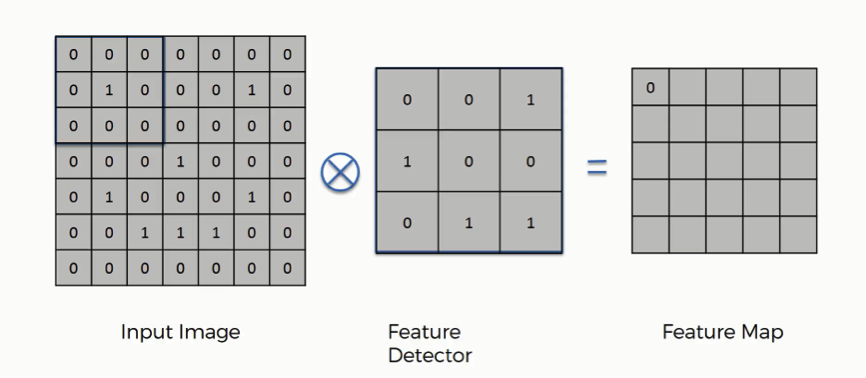
\includegraphics[width=3.5in]{figures/chapter4/convolution.png}
    \caption{Diagram showing the application of a single convolutional filter to a single window of an input image \cite{cnn_blog}.}
    \label{fig:conv}
\end{figure}

In the case of image processing, certain filters (referred to as feature detectors) can apply human interpretable image transformations as shown in Figure \ref{fig:ex_convs}. However, most learned convolutions are not meaningful to humans.\\

\begin{figure}[htb!]
    \centering
    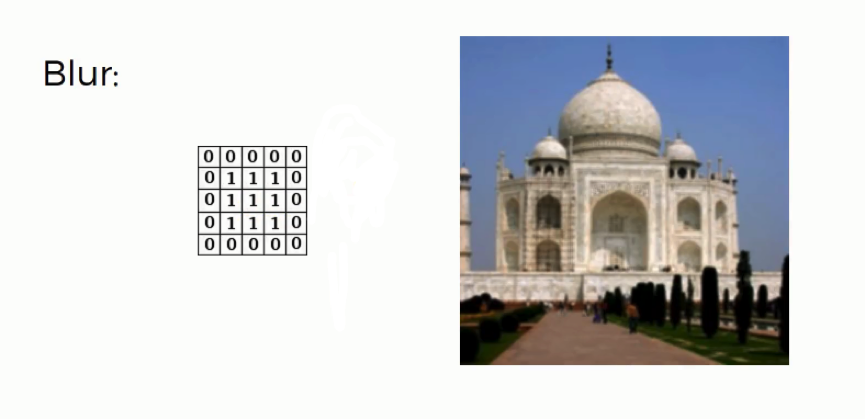
\includegraphics[width=2.5in]{figures/chapter4/blur_filter.png}\\
    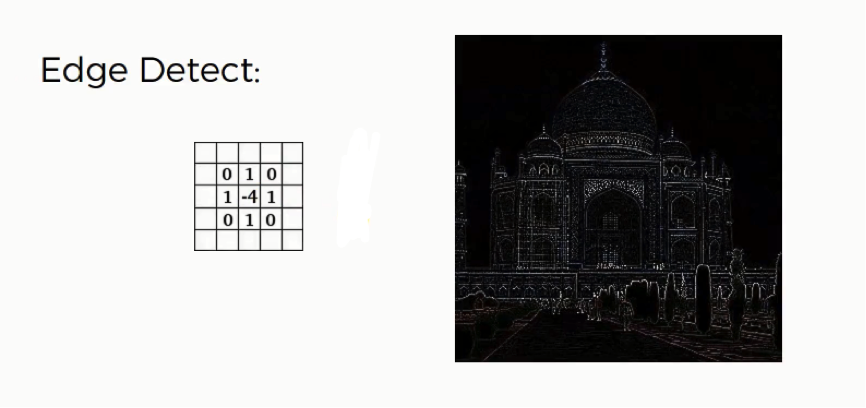
\includegraphics[width=2.5in]{figures/chapter4/edge_filter.png}
    \caption{Two examples of interpretable convolutional filters for image processing \cite{cnn_blog}.}
    \label{fig:ex_convs}
\end{figure}

Mathematically, the transfer of information from a convolutional layer is expressed as 
$$
h_{ij}=g(\mathbf{k}_j\cdot\mathbf{x}_i+b_j)
$$
\noindent where $\mathbf{k}_j$ is an individual filter and $i$ indexes the patches $\mathbf{k}_j$ is applied to. Applying the same filter in patches over the entire input image has a similar effect to weight-sharing in a standard NN. This reduces the number of learned parameters in the model and thus decreases training time. This also allows components of an input image to be recognized regardless of their position in the image.\\

Convolutional layers are typically followed by non-linear down-sampling layers called pooling layers, which reduce the dimensionality of the data by combining the outputs of nodes from the previous layer. Pooling is particularly important for image classification problems where the detection of individual image components often matters less than their spatial relation to other components. Pooling also reduces the memory usage and training time of CNNs. A common pooling method is max pooling where the maximum value in a certain window of the convolved input is passed to the next layer as shown in Figure \ref{fig:maxpool}.\\

\begin{figure}[htb!]
    \centering
    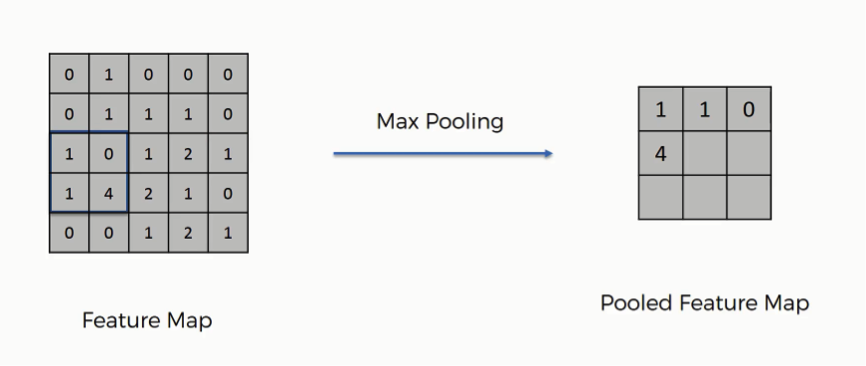
\includegraphics[width=3in]{figures/chapter4/maxpool.png}
    \caption{A graphical representation of max pooling \cite{cnn_blog}.}
    \label{fig:maxpool}
\end{figure}

CNNs usually contain many iterations of convolutional layers followed by pooling layers. This allows the model to learn a hierarchical representation of the training data moving from low- to mid- to high-level components. The series of convolutional and pooling layers can be followed by a flattening layer which compresses the convolved inputs into a 1D vector, and one or more fully connected layers that use the transformed input to complete the training task. An example of an entire image classification CNN incorporating all the components described above is shown in Figure \ref{fig:full_cnn}. CNNs can be trained with backpropagation just as standard NNs. 

\begin{figure}[htb!]
    \centering
    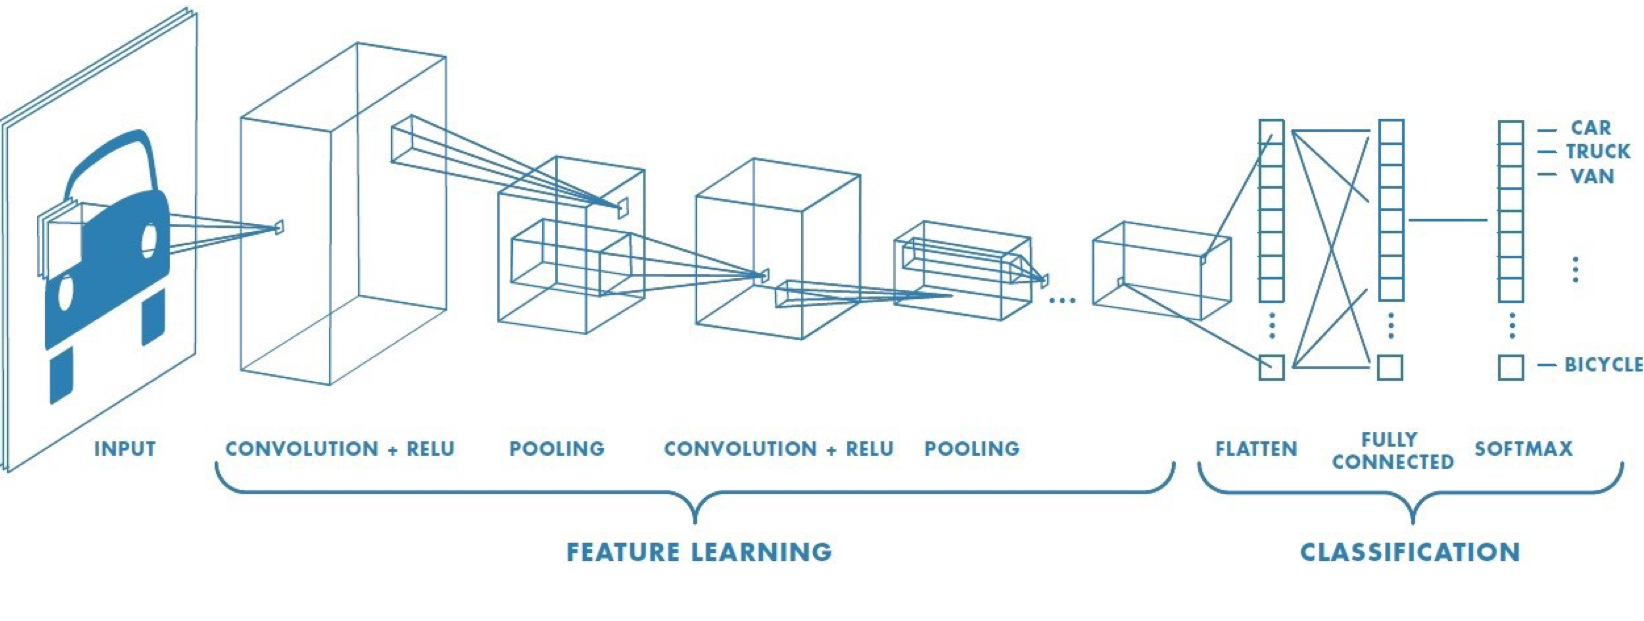
\includegraphics[width=4.5in]{figures/chapter4/full_cnn.png}
    \caption{Schematic depiction of a full convolutional neural network built for image classification.}
    \label{fig:full_cnn}
\end{figure}

\subsubsection{Recurrent NNs}
Neither standard NNs nor CNNs can handle variable length training data without altering certain data points by dropping information or adding dummy values. This functionality is critical for tasks like language processing or, in the case of HEP, allowing different numbers of clusters or tracks to contribute to object reconstruction. Additionally, neither type of network preserves order information of the inputs which is crucial for tasks like speech recognition or track-finding.\\

Recurrent nodes for NNs were developed in the 1980s to allow information preservation NN training and accommodate variable length inputs \cite{rnn_paper}. A basic recurrent node is described mathematically as 
$$
\mathbf{h}_i+1=g_i(W\mathbf{h}_i+V\mathbf{h}_{i-1}+\mathbf{b})
$$
\noindent where $W$ is the standard weight matrix connecting one layer to another and $V$ is the recurrent weight matrix that allows processed data to be fed back into the same layer. $h_{i-1}$ can represent either a previous feature or a previous time step. NNs containing one or more layers of recurrent nodes are referred to as Recurrent Neural Networks (RNNs); a simple, single layer RNN is shown in Figure \ref{fig:rnn}.\\  

\begin{figure}[htb!]
    \centering
    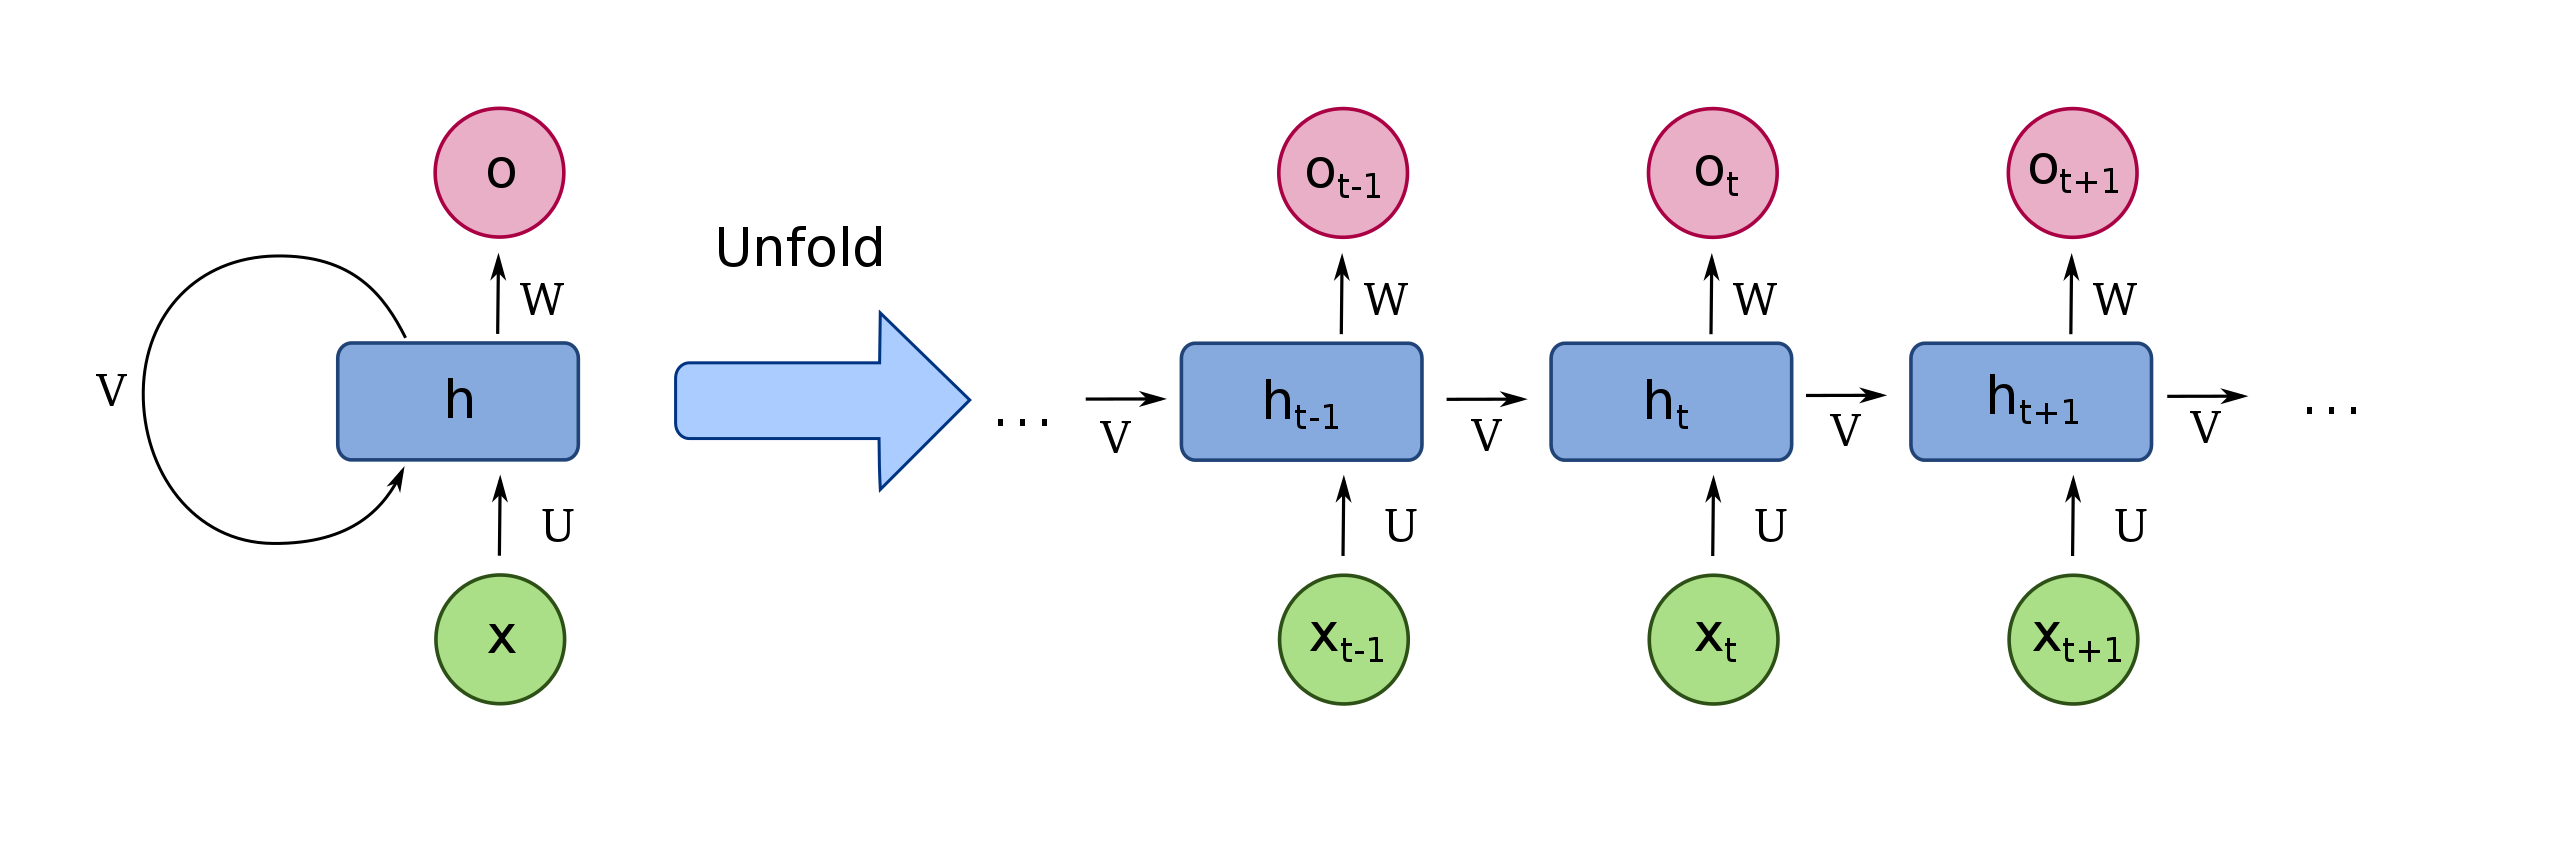
\includegraphics[width=5in]{figures/chapter4/rnn.png}
    \caption{A single layer recurrent neural network unfolded to show a series of time steps in data training.}
    \label{fig:rnn}
\end{figure}

In practice, deep RNNs tend to experience vanishing or exploding gradients which make it computationally difficult to preserve information from distant input features or time steps. In the past 20 years, different techniques have been developed to allow the training of deep RNNs. The most common technique is introducing gating to the recurrent nodes which allow the transformation matrices to be applied selectively. Long Term Short Term Memory Units (LSTMs) and Gated Recurrent Units (GRUs) are popular gated nodes. LSTMs, shown in Figure \ref{fig:lstm}, include three gates that control the flow of information withing the node. These are the input gate I, output gate O, and forget gate F. Each gate is parameterized by its activation function and its input and recurrent weight matrices $W$ and $V$. GRUs are simplified LSTMs with no output gates.\\

\begin{figure}[htb!]
    \centering
    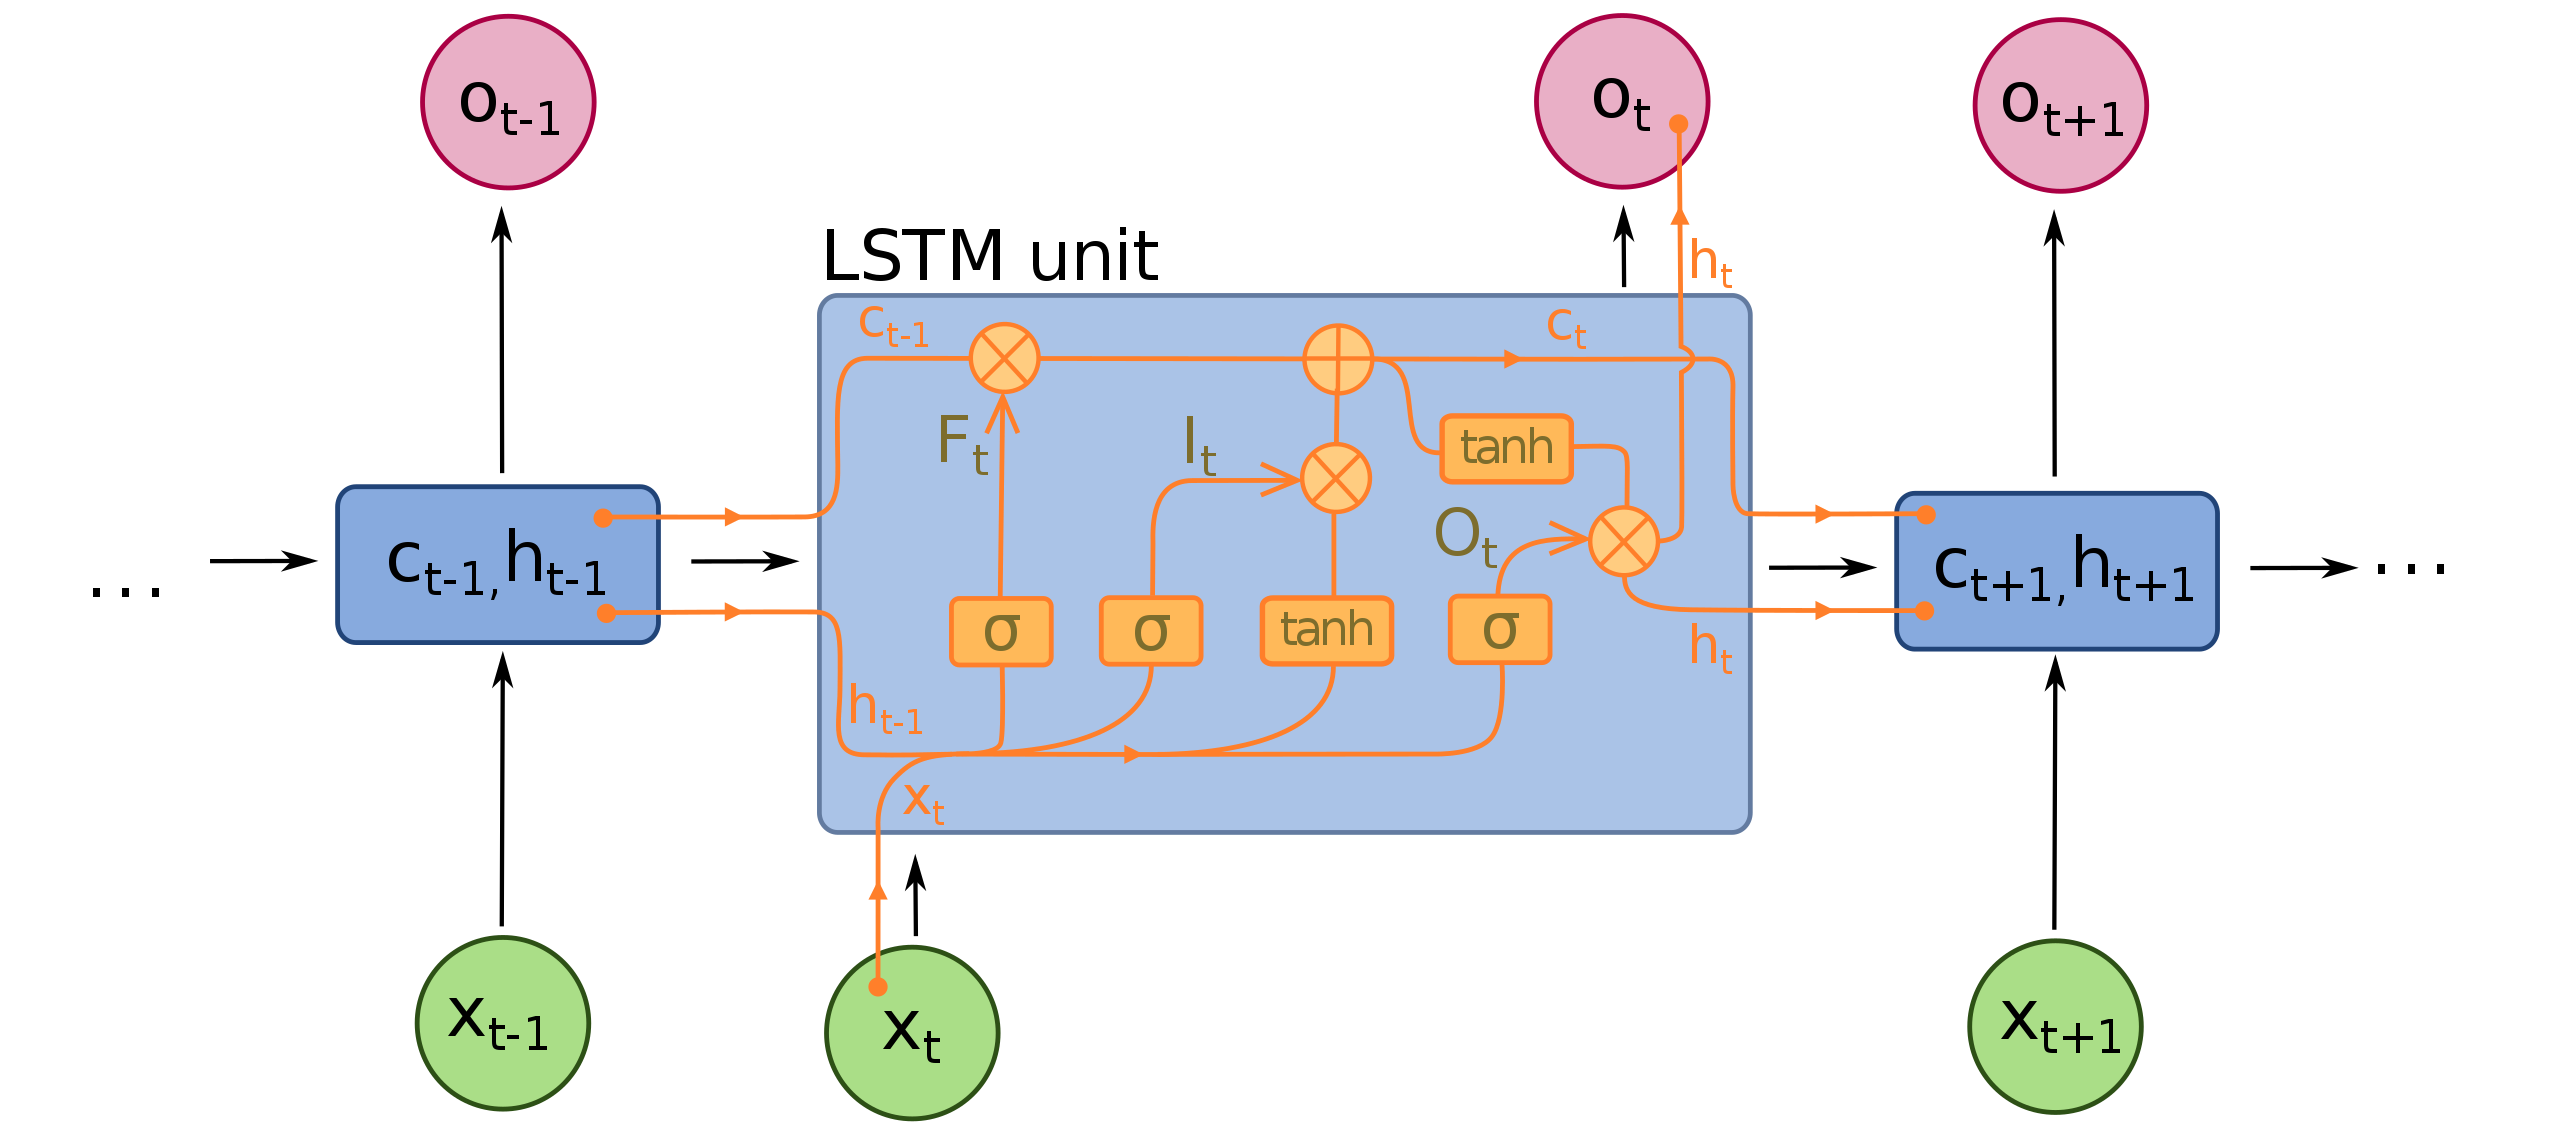
\includegraphics[width=4in]{figures/chapter4/lstm.png}
    \caption{A single LSTM node across three time steps. In this example, sigmoid and tanh activation functions are used and $c_i$ represents the previous state of information within the node.}
    \label{fig:lstm}
\end{figure}

\subsubsection{Adversarial Networks}
Unlike CNNs and RNNs, adversarial NNs do not introduce new node types to the standard NN but rather combine two NNs into a single classifier. This is done by pitting two networks against each other in a non-cooperative `game'. The primary network receives the training data as input and attempts to complete the primary algorithm task (e.g. classification). The adversary network receives the output of the primary network as input and attempts to predict something else (Figure \ref{fig:ann}). The two networks are trained together by combining their loss functions as $L=L_f(\mathbf{X})-L_r(f(\mathbf{X}),\mathbf{X})$ where $f$ refers to the primary network and $r$ refers to the adversary. Typically optimizing fully for both objects is impossible and a hyperparameter $\lambda$ is introduced to scale the importance of the adversary task in the loss function. 

\begin{figure}[htb!]
    \centering
    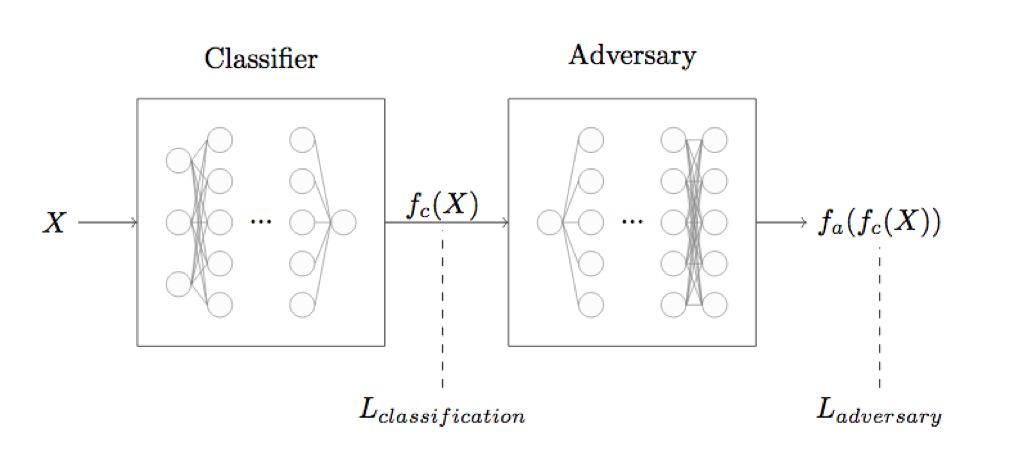
\includegraphics[width=3.5in]{figures/chapter4/ann.png}
    \caption{An example adversarial neural network where the primary task is classification \cite{pivot_paper}.}
    \label{fig:ann}
\end{figure}

Adversarial neural networks are commonly used to generate new data. In this case, the primary task is generating a new data point and the adversary task is predicting if the input data is real or generated. These types of networks are called Generative Adversarial Networks (GANs). Another common use of adversarial neural networks is to force a classifier to be robust to a certain feature of the training data which may not be explicitly included, but can nonetheless be constructed from the input features. In this case, the primary task is classification while the adversary task is predicting the feature of concern.\\

%% SEC: APPLICATIONS
\section{Applications in LHC Physics}\label{sec:apps}
Many computing tasks at various stages of the LHC computing flow (Chapter 3) rely on large volumes of high dimensionality data, which makes them appropriate use cases for a variety of ML algorithms. Implementing these algorithms come with the additional benefit of being able to utilize information that traditional cut-based methods cannot (i.e. variables whose distributions overlap and low-level information like detector outputs). ML can also reduce algorithm dependency on systematics like pile-up or simulation mis-modeling.\\

Furthermore, many ML algorithms, once trained, are faster to run than cut-based methods. Consequently, LHC physicists have already found many uses ML in detector trigger systems. This area of study is of particular importance for the development of the HL-LHC. Excellent surveys of the current status of ML for HEP research can be found in \cite{dan_paper}, \cite{hepml_site}, and \cite{ml_whitepaper} and primary LHC-based research areas are described below.

%subsec: IDs
\subsection{Reconstruction, Identification, and Calibration}
Particle and event reconstruction, identification, and calibration is the focus of a great deal of LHC-based ML research. Many of these tasks can be formulated as classification problems making them excellent candidates for supervised learning models. 

\subsubsection{BDTs and Standard NNs}
Many of the cut-based methods originally developed for these tasks make use of physics-motivated constructed variables, making them a natural use case for BDTs and NNs. Additionally, these methods are relatively easy to understand and develop; thus they were the focus of initial LHC ML research.\\

An excellent example of BDTs and NNs for particle ID the study of W- and top-jet tagging in ATLAS \cite{w_top_bdt_paper}. Here, W-jets and top-jets refer to jets originating from Ws or tops that are `fat' (large radius) or boosted so as to be reconstructed as a jet rather than individual decay products. The training data-set was constructed by reconstructing jets in MC samples with the standard anti-$k_t$ clustering, reconstructing `truth-jets' using truth-level information of long-lived particles, and then matching the clustered jets and truth-jets to form a labeled data-set. The BDTs and NNs were trained using standard physics-motivated jet substructure variables where the final set of variables was chosen through an iterative process. Both algorithms were optimized with a hyperparameter grid search and tested for over-training with cross-validation. As shown in Figure \ref{fig:wtop_bdt_plots}, both the BDTs and NNs outperform the previous cut based method. Similar studies for other ID tasks are summarized in \cite{ben_jet_paper}.\\ 

\begin{figure}[htb!]
        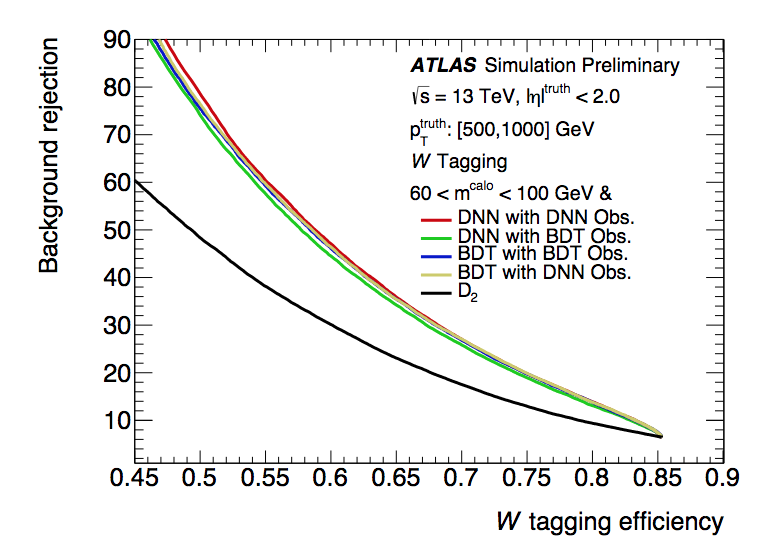
\includegraphics[width=2.8in]{figures/chapter4/w_top_bdt_weff.png}
        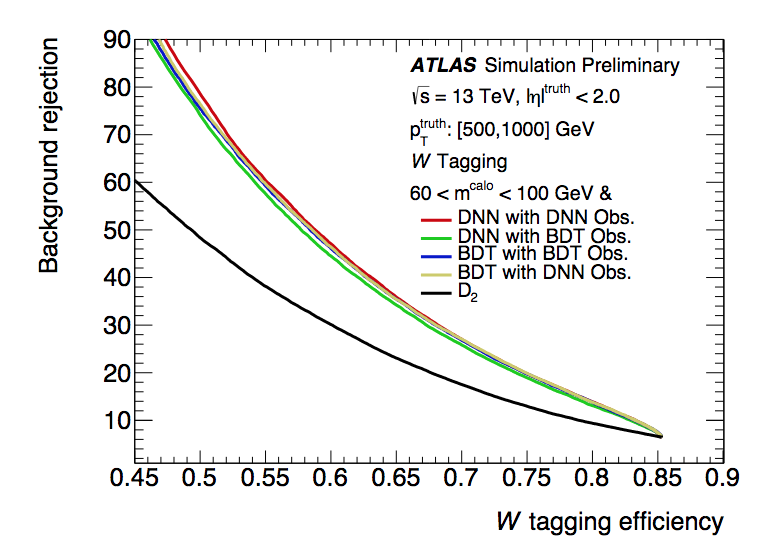
\includegraphics[width=2.8in]{figures/chapter4/w_top_bdt_weff.png}
    \caption{Performance of BDTs and deep NNs (DNNs) for W-jet tagging (left) and top-jet tagging (right). For both plots the black curve represents the standard cut-based method \cite{w_top_bdt_paper}.}
    \label{fig:wtop_bdt_plots}
\end{figure}

Track-reconstruction for LHC experiments is highly CPU and time intensive. ML has already found some use in current tracking methods; for example, in ATLAS NNs are used to assign track energies in the case where multiple tracks pass through the same pixel cluster \cite{track_nn}. Nonetheless, the most CPU intensive portion of track finding is the initial track candidate seeding. As described in Chapter 3, in ATLAS this is currently done with a Kalman filter; unfortunately this is impractical in terms of computing needs and decreasing accuracy in the high pileup environment of the HL-LHC. Many on-going research projects seek to solve this problem, including crowd-sourced computing challenges like \cite{track_kaggle}.\\

Adjusting the weights of MC events to better match data distributions and correcting the assigned energy of reconstructed objects are important tasks in LHC computing flows. Typically this is done by calculating a re-weighting factor by comparing data and MC in the first case or reconstructed and truth jets in the latter case. Studies like \cite{bdt_reweight} have shown that using BDTs for MC re-weighting is both faster and more accurate; in fact, discriminators have a more difficult time distinguishing between ML re-weighted MC and data than between data and previous MC re-weighting techniques. BDT-based calibration is implemented for many physics objects in ATLAS (e.g. electrons and photons \cite{bdt_calibration}) with excellent performance.

\subsubsection{Images and CNNs}\label{sec:cnn_ids}
In 2014, the process of representing jets as images was developed \cite{jetimages1}. Cells or towers in a detector calorimeter are represented as individual pixels and the value of the pixel is the amount of energy deposited in that cell/tower. In practice, this representation requires some amount of pre-processing to account for detector geometry and image sparsity. This typically involves noise reduction, ROI finding to select a certain window of cells to represent, cell geometry normalization, and alignment to exploit detector $\eta-\phi$ symmetry. Additionally, most jet images studies have focused on jets only in the barrel region to avoid the granularity differences between the barrel and endcap calorimeters. A composite of several pre-processed W-jet images is shown in Figure \ref{fig:jet_image}.

\begin{figure}[htb!]
    \centering
    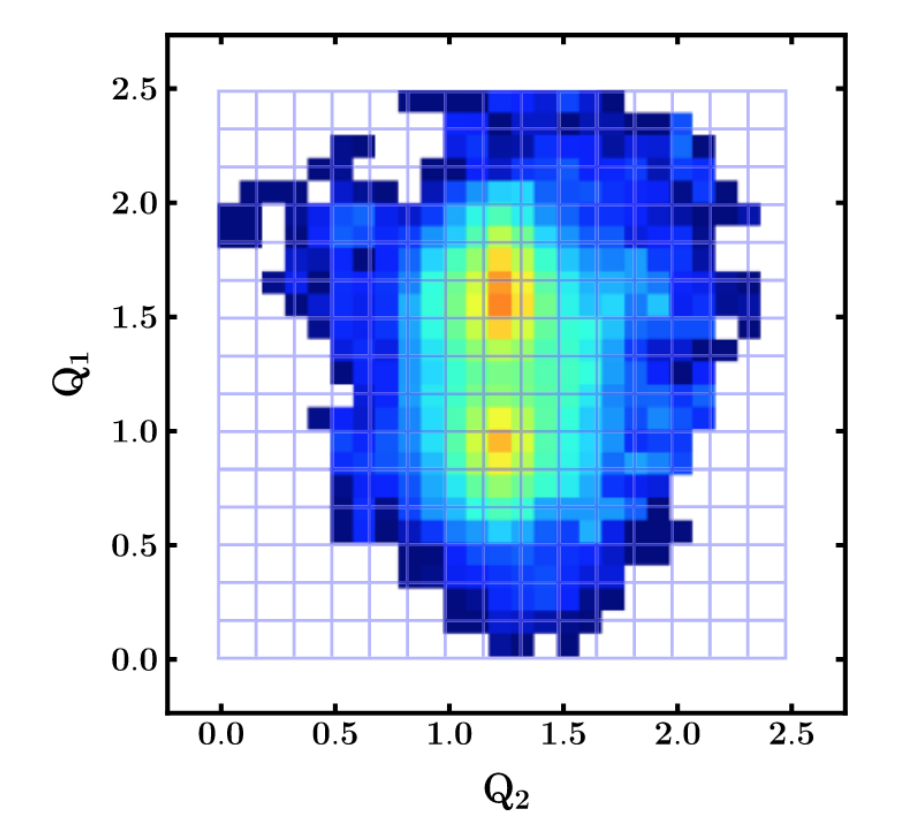
\includegraphics[width=3.5in]{figures/chapter4/jet_image.png}
    \caption{Average of several pre-processed W-jet images. Here the $Q_1$ and $Q_2$ axes represent the transformed $\eta-\phi$ space \cite{jetimages1}.}
    \label{fig:jet_image}
\end{figure}

There are numerous studies of image-based jet classification using CNNs \cite{ben_jet_paper}. One of the most successful studies sought to distinguish W-jets from background QCD-jets \cite{wqcd_jetimages} using a CNN with ReLu activations and a `Max-Out' network that consisted of two max pooling layers and two fully connected layers. Both networks were trained with 8 million samples and an additional 2 million test samples generated using Pythia and pre-processed as described above. Additionally, both networks were optimized using a limited hyperparameter grid search. As shown in Figure \ref{fig:wqcd_jetimages}, both network types outperformed cut-based combinations of standard jet substructure variables.\\

\begin{figure}[htb!]
    \centering
    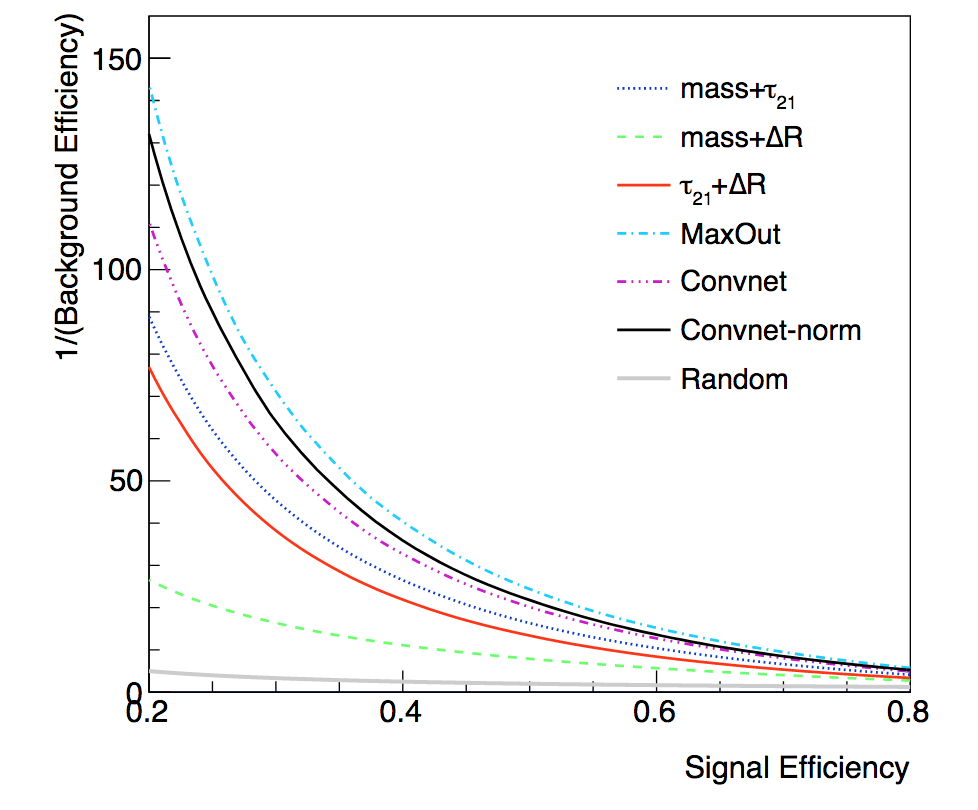
\includegraphics[width=4in]{figures/chapter4/wqcd_jetimages_results.png}
    \caption{Performance comparison of CNNs (purple dashed and black curves), a Max-Out network (blue dashed curve) and cut-based discrimators using jet substructure variables (red, blue dotted, and green dashed curves) on the W- vs QCD-jet discrimination task \cite{wqcd_jetimages}.}
    \label{fig:wqcd_jetimages}
\end{figure}

This method is also being studied for electron ID in the EM calorimeter as described in Chapter 5. 

\subsubsection{RNNs}
RNNs have been used in a variety of particle ID and tagging applications at the LHC. These methods are advantageous because they allow the input of variable length track and cluster lists, thus allowing maximal information preservation. Successful examples include boosted top-tagging \cite{top_rnn}, ATLAS b-tagging \cite{rnn_bottom}, and the new ATLAS RNN tau ID and trigger \cite{tau_rnn}.\\

Language processing inspired RNNs have found uses in jet clustering \cite{qcd_clustering}. This method relies on the physically motivated assumption that the particles produced in a jet should be formed in some QCD-dictated order. In this application, the RNN takes the 4-momenta of particles in an event as input and recursively learns an embedded representation of the jets in the event that is then classified by a fully-connected NN (Figure \ref{fig:rnn_jet_cluster}). In the same W- vs QCD-jet tagging task described in Section \ref{sec:cnn_ids} jets constructed and classified with this method achieved the same accuracy as the Max-Out network but required substantially less training time.

\begin{figure}[htb!]
    \centering
    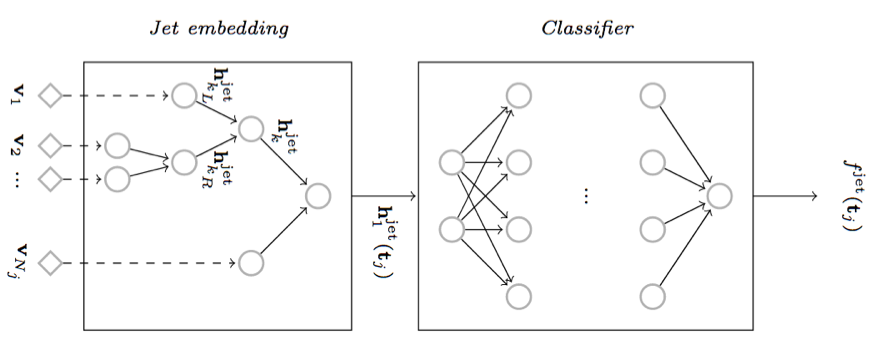
\includegraphics[width=4.5in]{figures/chapter4/rnn_jet_cluster.png}
    \caption{Schematic of QCD-motivated RNN-based jet-clustering and classification \cite{qcd_clustering}.}
    \label{fig:rnn_jet_cluster}
\end{figure}

%subsec:Analyses
\subsection{Analyses}
ML, particularly NNs, has been utilized to improve the event selection efficiency and background rejection for a range of LHC analyses. One of the earliest studies used NNs to select events containing different exotic particles. This study compared a shallow NN trained on `high-level' features (i.e. reconstructed boson masses, MET, etc) to a deep NN trained on the same high-level features and a deep NN trained on `low-level' features (i.e. individual particle $p_T$, number of jets, etc) \cite{nn_exotic_particles}. As shown in Table \ref{tab:exotic_higgs_table}, the deep NN trained on low-level features outperformed the networks trained on physics-motivated variables, indicating that some information is lost in the construction of these variables.\\

\begin{table}[htb!]
    \centering
    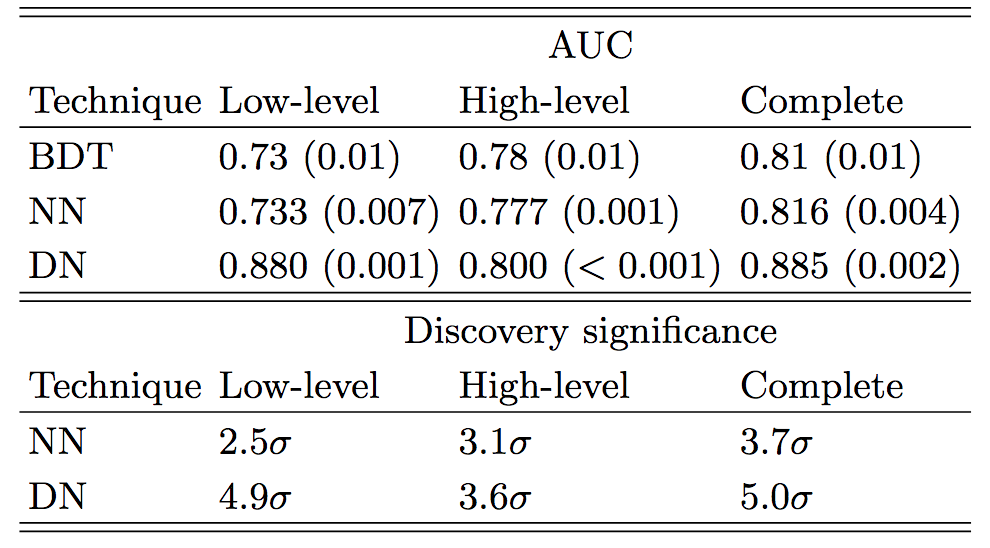
\includegraphics[width=3in]{figures/chapter4/exotic_higgs_table.png}
    \caption{Performance for the various event selection algorithms trained to select exotic Higgs events. NN refers to the shallow NN, DN refers to the deep NN, and complete means the combination of high-level and low-level features \cite{nn_exotic_particles}.}
    \label{tab:exotic_higgs_table}
\end{table}

Deep NNs have been used in various other LHC searches and analyses. However, these methods do not always yield higher signal selection efficiency or improved background rejection. The usefulness of these methods depends on the specific analysis and is an on-going area of research. 

\subsubsection{$ZZ_d\rightarrow llll$ Search}
ML event classification has also been studied to improve the selection efficiency in the ATLAS Run-2 $H\rightarrow\ ZZ_d \rightarrow llll$ search. This search targets a massive mediator of the hypothetical $U(1)_d$ dark gauge symmetry extension of the SM \cite{zzd_paper}. In contrast to related dark photon searches that rely on measuring displaced vertices or MET \cite{dark_photon_paper}, the massive nature of the $Z_d$ allows the use of the Higgs as a portal to this dark sector. This is analysis selects $H\rightarrow ZZ^* \rightarrow llll$ events and fits the $Z^*$ reconstructed mass spectrum. If no $Z_d$ boson exists, this mass spectrum would be flat, but if the $Z_d$ does exists, there will be an excess at the mass of the $Z_d$.\\

Efficiently selecting $H\rightarrow ZZ^* \rightarrow llll$ events is thus critical for increasing the sensitivity of this search. An initial Run-2 study explored using BDTs and NNs for event selection in an effort to improve efficiency. An extensive variable optimization study was conducted to select the training features; the final BDT was trained with $p_T^{4l}$, $\eta^{4l}$, and $p_T^{Z_2}$. The NN was trained with the same variables as the Run-1 cut-based analysis and a grid search over all hyperparameters was used to optimize the network architecture. The potential performance of a Run-2 cut-based selection was modeled using the rectangular cut functionality of TMVA built with the Run-1 variables. As shown in Figure \ref{fig:zzd_roc}, both ML methods out-performed the cut-based method. 

\begin{figure}[htb!]
    \centering
    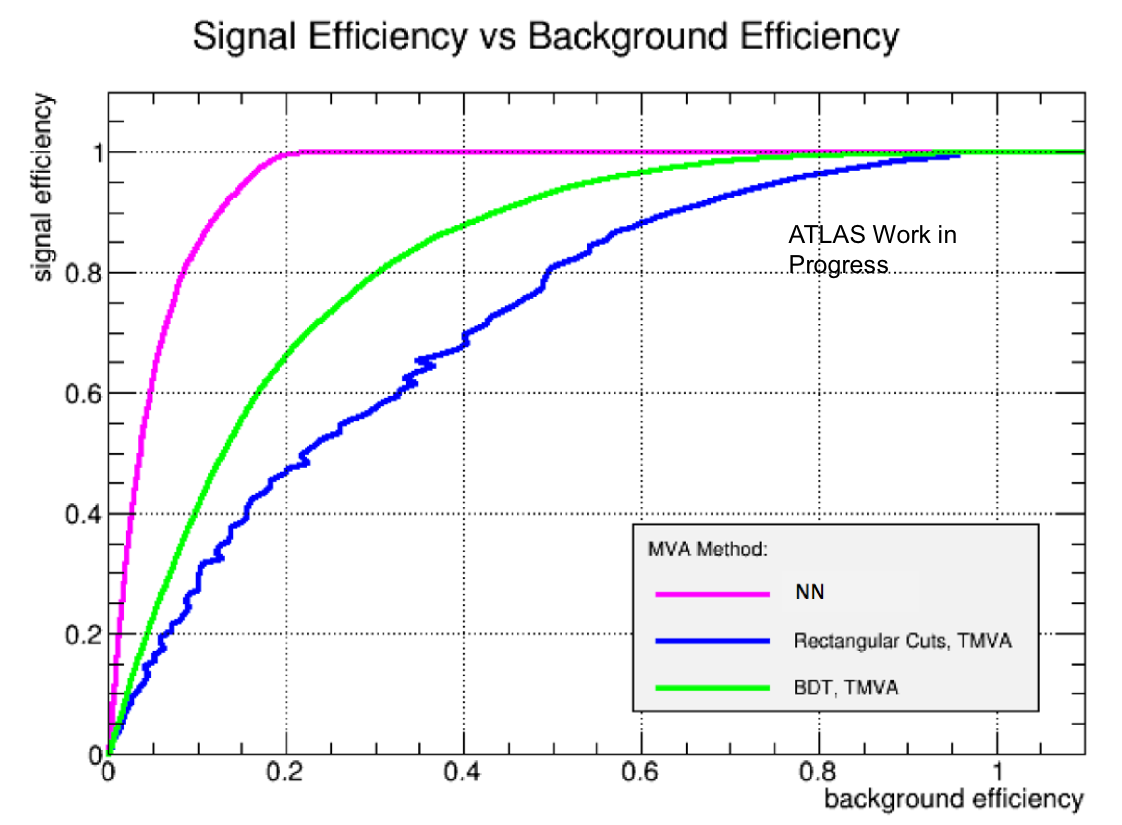
\includegraphics[width=4in]{figures/chapter4/zzd_roc.png}
    \caption{ROC-curve comparison of $H\rightarrow ZZ^* \rightarrow llll$ event selection algorithms performance.}
    \label{fig:zzd_roc}
\end{figure}

%subsec: Simulation
\subsection{Simulation}
As described in Chapter 3, detector simulation is the most computationally intensive component of the ATLAS simulation chain. ML,  particularly GANs, have been shown to help speed up the this process for some detector-object interactions by generating images like those introduced in Section \ref{sec:cnn_ids}. In these methods, the primary task is generating a new detector image and the adversary task is discriminating between images generated with the full detector simulation and images generated by the primary network. A common issue when training GANs is so-called `mode-collapse' where the generator learns a small feature that is maximally confusing to the adversary and thus does not produce a variety of simulated examples. Mode-collapse can be alleviated by introducing a third network trained to complete some auxiliary task and incorporating its error into the overall loss function.\\

Location-aware GANs (LAGANs), which introduce locally connected layers to preserve location information, have been successfully used to generate jet images \cite{jet_gan}. This implementation included an auxiliary task of distinguishing W-jets from QCD-jets. As shown in Figure \ref{fig:lagan_plots}, the LAGAN produced images with kinematic information that closely matched those produced by Pythia. Furthermore, the LAGAN simulation was an order of magnitude faster that the Pythia simulation. Reducing the computing load for MC simulation is critical to ensure successful physical analyses in the HL-LHC. A similar method was successful in generating electromagnetic calorimeter shower images \cite{em_gan}. 

\begin{figure}[htb!]
    \centering
    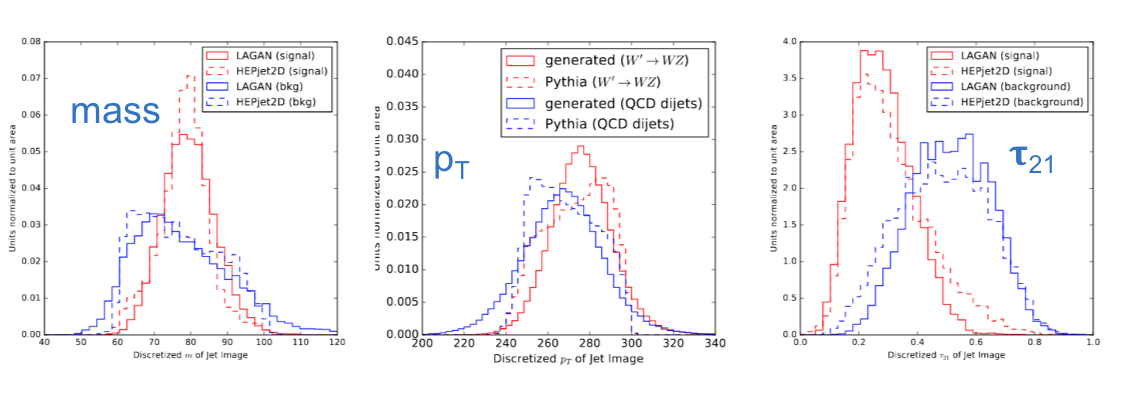
\includegraphics[width=5in]{figures/chapter4/lagan_plots.png}
    \caption{Comparison of LAGAN generated (solid lines) and Pythia generated (dotted lines) jet kinematics (jet mass (left), (jet $p_T$ (center), and n-subjettiness (right)) for signal (W-jets, red lines) and background (QCD jets, blue lines) \cite{jet_gan}.}
    \label{fig:lagan_plots}
\end{figure}

%subsec: Systematics 
\subsection{Systematics}
A central challenge in many LHC analyses is robustness of results to systematic uncertainties and changing conditions. Adversarial networks can also be used to impose physics motivated constraints (such as reducing pileup dependence or decorrelating classification results from some variable) on NN-based classifiers. In these cases, the primary task is the specific classification and the adversary task is to reproduce the feature of interest. This can be formulated mathematically by rewriting the underlying model of features $X$ and labels $Y$ as $p(X,Y,Z)$ where $Z$ is a nuisance parameter and $Y$ now depends on both $X$ and $Z$. The goal of the network is then to find a function $f_{\phi}(X)=Y$ that is robust to the unknown value of $Z$. This typically results in a less accurate classifier, but has the advantage of reducing uncertainty on the final measurement.\\

The first use of this method for LHC physics used a simplified quantization of pileup as the nuisance parameter; $Z$ could take on two discrete values: $Z=0$ for no pileup and $Z=1$ for a pileup of 50 \cite{pivot_paper}. Figure \ref{fig:pivot_plot} shows the approximate median significance (AMS) of the final classification as a function of the selected decision threshold for a variety of adversary importance weights ($\lambda$). The network with $\lambda=10$ achieves the highest significance, illustrating the advantages of some sacrifices in classifier accuracy for reducing pileup dependence.\\

\begin{figure}[htb!]
    \centering
    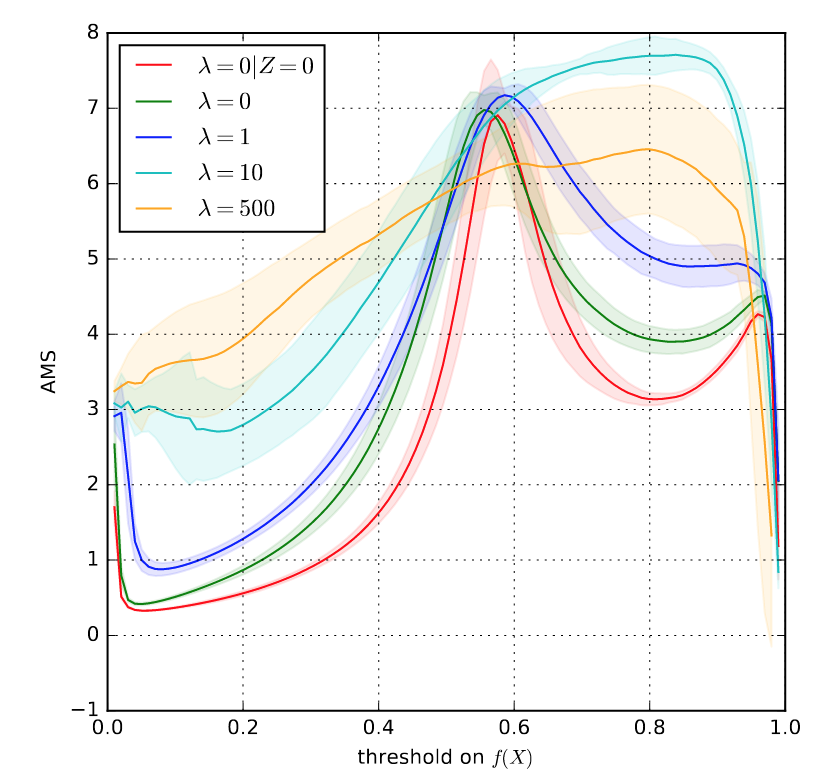
\includegraphics[width=3.5in]{figures/chapter4/pivot_an_plot.png}
    \caption{Approximate median significance as a function of decision threshold for networks trained with different values of $\lambda$ \cite{pivot_paper}.}
    \label{fig:pivot_plot}
\end{figure}

Another study sought to decorrelate the output of jet classifiers from jet mass \cite{jet_decorr}. This is useful because many current jet taggers distort the jet mass distribution which increases the uncertainty of background models in many analyses thereby decreasing the final result significance. In this study, the primary task was distinguishing W-jets from QCD-jets and the adversary task was reproducing the jet mass. This study also found improved final significance when sacrificing some classification power in favor of reducing jet mass dependence, even when compared to non-ML methods for preventing distortions of the jet mass spectrum.

\pagebreak

It is clear that there are substantial opportunities to improve physics results at the LHC using ML. The following chapters detail additional studies applying ML to electron ID and the $VH,H\rightarrow\tau\tau$ analysis.

%\subsubsection{Interpretability}
%pros and cons
%- deep learning from dan paper
%-lessens the need for physically engineered variables, but not satisfactory
%- diffucult to interpret answer
%- more difficult to communicate and publish 
%w vs qcd jet
%gans